\documentclass{article}
\usepackage{amsmath}
\usepackage[mathletters]{ucs}
\usepackage[utf8x]{inputenc}
\usepackage[margin=1.5in]{geometry}
\usepackage{enumerate}
\newtheorem{theorem}{Theorem}
\usepackage[dvipsnames]{xcolor}
\usepackage{pgfplots}
\setlength{\parindent}{0cm}
\usepackage{graphics}
\usepackage{graphicx} % Required for including images
\usepackage{subcaption}
\usepackage{bigintcalc}
\usepackage{pythonhighlight} %for pythonkode \begin{python}   \end{python}
\usepackage{appendix}
\usepackage{arydshln}
\usepackage{physics}
\usepackage{tikz-cd}
\usepackage{booktabs} 
\usepackage{adjustbox}
\usepackage{mdframed}
\usepackage{relsize}
\usepackage{physics}
\usepackage[thinc]{esdiff}
\usepackage{fixltx2e}
\usepackage{esint}  %for lukket-linje-integral
\usepackage{xfrac} %for sfrac
\usepackage{hyperref} %for linker, må ha med hypersetup
\usepackage[noabbrev, nameinlink]{cleveref} % to be loaded after hyperref
\usepackage{amssymb} %\mathbb{R} for reelle tall, \mathcal{B} for "matte"-font
\usepackage{listings} %for kode/lstlisting
\usepackage{verbatim}
\usepackage{graphicx,wrapfig,lipsum,caption} %for wrapping av bilder
\usepackage{mathtools} %for \abs{x}
\usepackage[norsk]{babel}
\definecolor{codegreen}{rgb}{0,0.6,0}
\definecolor{codegray}{rgb}{0.5,0.5,0.5}
\definecolor{codepurple}{rgb}{0.58,0,0.82}
\definecolor{backcolour}{rgb}{0.95,0.95,0.92}
\pagecolor[rgb]{0.075,0.075,0.075} \color[rgb]{1,1,1} %TODO: Slett når ferdig%
\lstdefinestyle{mystyle}{
    backgroundcolor=\color{backcolour},   
    commentstyle=\color{codegreen},
    keywordstyle=\color{magenta},
    numberstyle=\tiny\color{codegray},
    stringstyle=\color{codepurple},
    basicstyle=\ttfamily\footnotesize,
    breakatwhitespace=false,         
    breaklines=true,                 
    captionpos=b,                    
    keepspaces=true,                 
    numbers=left,                    
    numbersep=5pt,                  
    showspaces=false,                
    showstringspaces=false,
    showtabs=false,                  
    tabsize=2
}

\lstset{style=mystyle}
\author{Oskar Idland}
\title{FYS2140 - Oblig 3}
\date{}
\begin{document}
\maketitle
\newpage

\section*{\underline{A Diskusjonsoppgaver}}
\subsection*{Oppgave 1}
\subsubsection*{a)}
En bil med høy fart har høyere bevegelsesmengde $p$ enn en fotgjenger. Da får den en en lavere bølgelengde. 
\subsubsection*{b)}
Når bilen stopper vil bevegelsesmengden gå mot null og bølgelengden vil gå mot uendelig. Dette gir også mening i kontekst av Heisenberg's usikkerhetsprinsipp ettersom vi vet den nøyaktig posisjonen må bølgelengden være udefinert. 

\subsection*{Oppgave 2}
\subsubsection*{a)}
Når en ikke gjør en observasjon på elektronene vil det likevel oppstå et interferensmønster selv om vi skyter ett og ett elektron gjennom spaltene. Dette er en bølgeegenskap. Når vi gjør en observasjon av én av spaltene for å se om elektronet passerer gjennom her vil vi ikke lenger se et interferensmønster. Da oppfører elektronet seg som om det var en partikkel.  

\subsubsection*{b)}
Som nevnt i oppgave 2a vil vi ikke lenger se et interferensmønster når vi gjør en observasjon av én av spaltene. Dette er fordi observasjonen kollapser bølgefunksjonen og gjør at vi observerer en partikkel. 

\section*{\underline{B Regneoppgaver}}
\subsection*{Oppgave 3}
En de Broglies-bølgelengde $λ$ er gitt ved 
\[
λ = \frac{h}{p}
\]
hvor $p$ er gitt ved
\[
p = \sqrt{\frac{E^2}{c^2} - m^2c^2}
\]


\subsection*{Oppgave 4}
\subsubsection*{a)}
Vi bruker at vi kan se på elektronet som både en partikkel og en bølge. 
\[
E_{\text{bølge}} = ℏw \quad , \quad p_{\text{rel. partikkel}} = \frac{1}{c} \sqrt{E^2 - \left(mc^2\right)^2} = p_{\text{bølge}} = ℏk
\]
Vi setter in utrykket for $E$ i utrykket for $p$. 
\[
\frac{1}{c} \sqrt{ℏ^2 w^2 - \left(mc^2\right)^2} = ℏk
\]
\[
h^2ω^2 = c^2ℏ^2k^2 + \left(mc^2\right)^2
\]
\[
ω = c\sqrt{k^2 + \left( \frac{mc}{ℏ} \right) ^2}
\]
\subsubsection*{b)}
\[
v_f = \frac{ω}{k} = c \sqrt{1 + \left( \frac{mc}{ℏk} \right) ^2}
\]
\[
v_g = \frac{\mathrm{d}ω}{\mathrm{d}k} = \frac{ck}{\sqrt{\frac{c^2m^2}{ℏ^2} + k^2}} = \frac{c}{\sqrt{1 + \left( \frac{mc}{ℏk} \right)^2}}
\]
\[
v_g ⋅ v_f = \frac{c}{\sqrt{1 + \left( \frac{mc}{ℏk} \right) ^2}} ⋅  c \sqrt{1 + \left( \frac{mc}{ℏk} \right) ^2} = c^2
\]

\subsubsection*{c)}
Relativitets teorien viser at ingenting kan reise raskere enn lysets hastighet. Det stemmer likevel ettersom $v_f$ er hastigheten bølgetoppene reiser gjennom mediet. Partikkelen selv reiser i gruppehastigheten $v_g$ som alltid er lavere enn lysets hastighet. 

\subsection*{Oppgave 5}
\subsubsection*{a)}
Vi løser oppgaven numerisk og får resultatet sett i \ref{fig: 5a}. Resultatet er at ettersom funksjonene har relativt lik fase vil det ta mange svingninger før bølgene går inn og ut av fase med hverandre. 
\begin{figure}[h!]
  \centering
  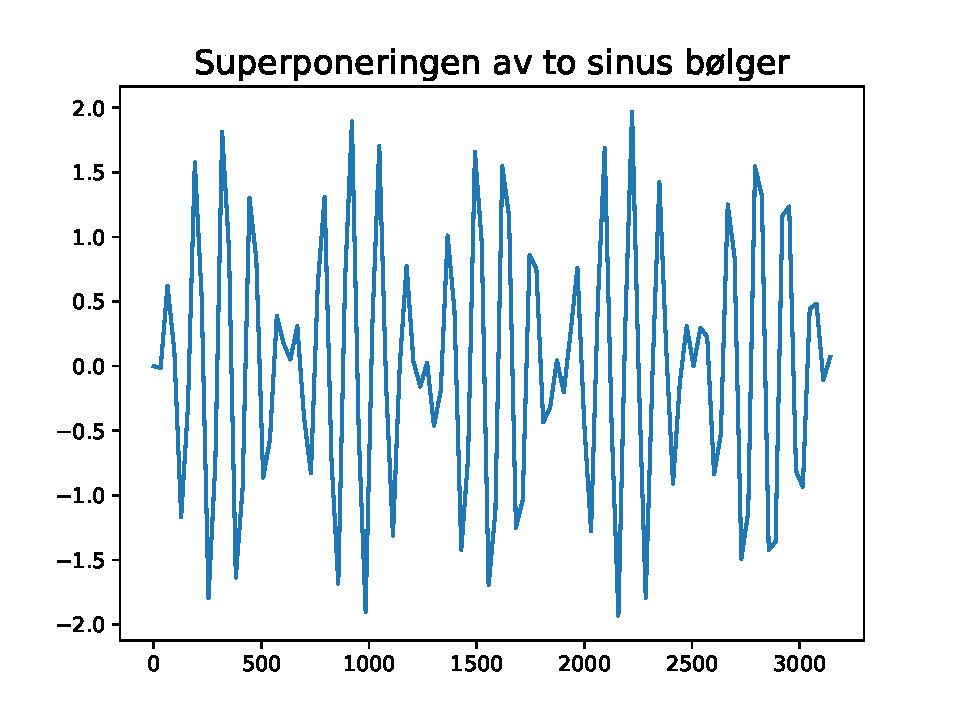
\includegraphics[width = \textwidth]{fig/5a.pdf}
  \caption{Oppgave 5.a}
  \label{fig: 5a}
\end{figure}

\subsubsection*{b)}
Vi definerer $ω, v_f$ og $v_g$ på følgende måte: 
\[
ω(k) = c\sqrt{k^2 + \left( \frac{mc}{ℏ} \right) ^2} \quad , \quad v_f = \frac{ω}{k} \quad , \quad v_g = \frac{\mathrm{d}w}{\mathrm{d}k} = \frac{k}{\sqrt{k^2 + 1}}
\]
hvor $m = c = ℏ = 1$. Vi løser dette numerisk og får at $v_f = 3.69$ og $v_g = 1.09$
\subsubsection*{c)}  
Ved å legge 1000 cosinus bølger oppå hverandre får vi følgende funksjon sett i 
\ref{fig: 5c}
\begin{figure}[h!]
  \centering
  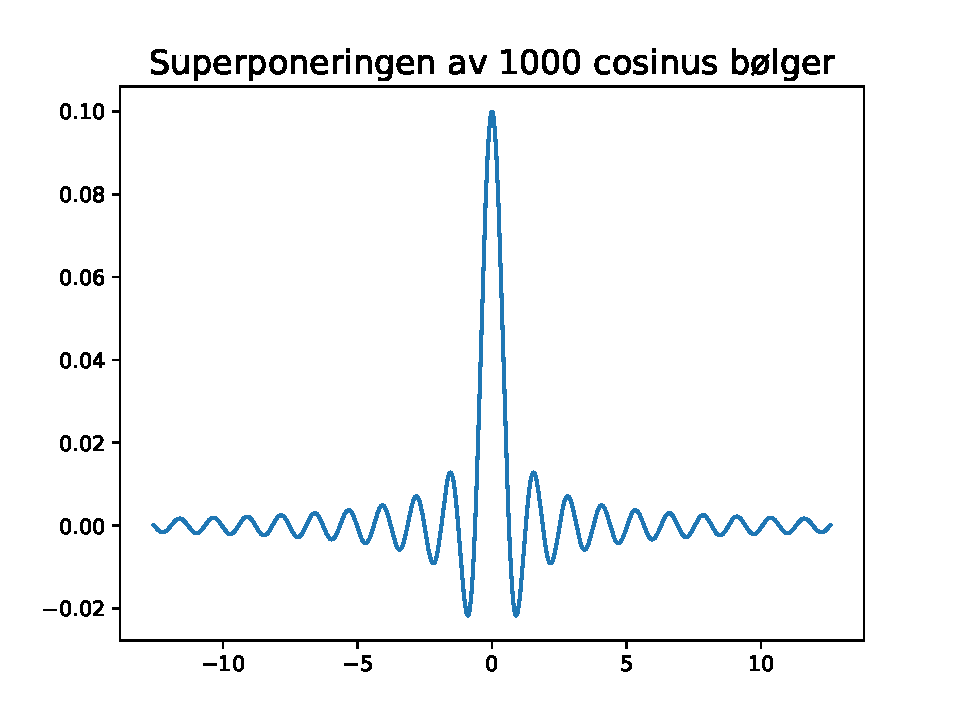
\includegraphics[width = \textwidth]{fig/5c.pdf}
  \caption{Oppgave 5.c}
  \label{fig: 5c}
\end{figure}
\end{document}